% Diagram: V9.0 Bound-Screaming Map + Two-Basin Parameter Consensus
% Top panel: which parameters are at bounds (bar chart)
% Bottom panel: Basin A vs Basin B parameter spreads (small multiples)
\documentclass{article}
\usepackage{tikz}
\usepackage[paperwidth=34cm,paperheight=24cm,margin=0.5cm]{geometry}
\pagestyle{empty}

\begin{document}
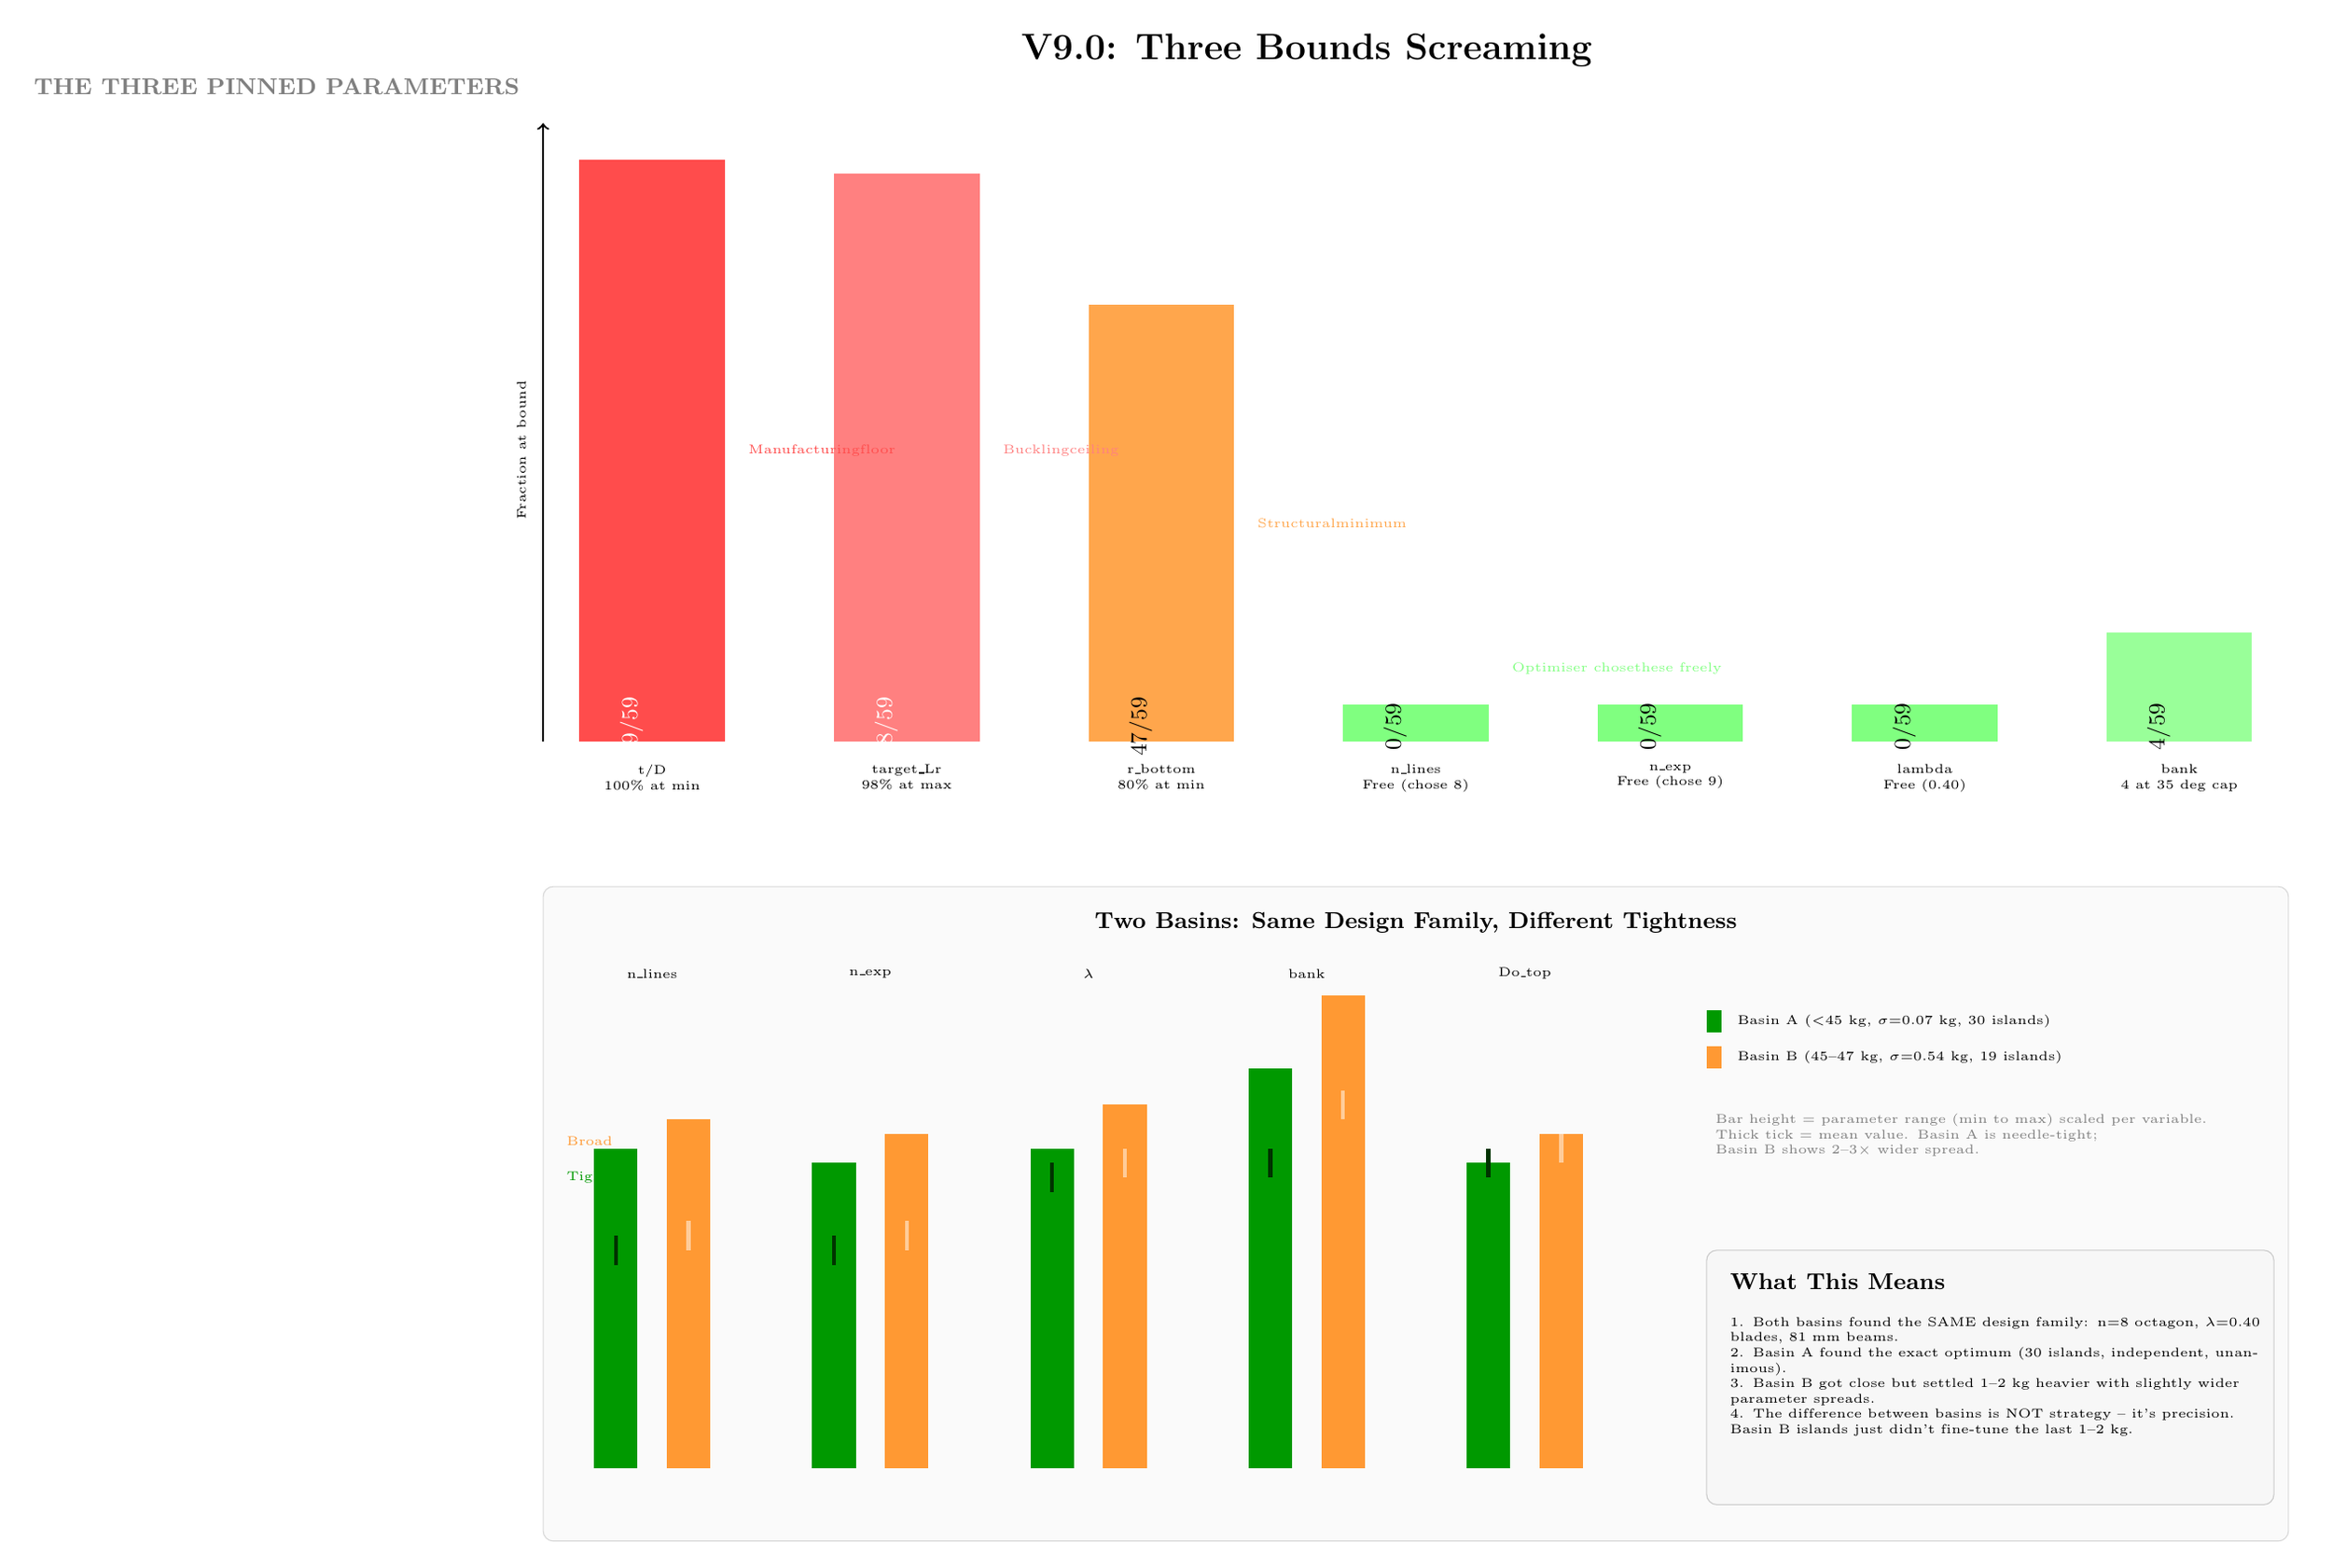
\begin{tikzpicture}[scale=1.0]

% ── TOP PANEL: Bound-screaming bar chart ──
% Title
\node[font=\Large\bfseries] at (11, 13.5) {V9.0: Three Bounds Screaming};

% Bars: fraction of 59 islands at bound
% t_over_D: 59/59 = 100%
\fill[red!70] (1.0, 4.0) rectangle (3.0, 12.0);
\node[font=\small, rotate=90, anchor=south, white] at (2.0, 4.2) {59/59};
\node[font=\tiny, anchor=north, text width=2cm, align=center] at (2.0, 3.8) {t/D\\100\% at min};

% target_Lr: 58/59 = 98%
\fill[red!50] (4.5, 4.0) rectangle (6.5, 11.8);
\node[font=\small, rotate=90, anchor=south, white] at (5.5, 4.2) {58/59};
\node[font=\tiny, anchor=north, text width=2cm, align=center] at (5.5, 3.8) {target\_Lr\\98\% at max};

% r_bottom: 47/59 = 80%
\fill[orange!70] (8.0, 4.0) rectangle (10.0, 10.0);
\node[font=\small, rotate=90, anchor=south] at (9.0, 4.2) {47/59};
\node[font=\tiny, anchor=north, text width=2cm, align=center] at (9.0, 3.8) {r\_bottom\\80\% at min};

% n_lines: 0/59 at bound (free)
\fill[green!50] (11.5, 4.0) rectangle (13.5, 4.5);
\node[font=\small, rotate=90, anchor=south] at (12.5, 4.2) {0/59};
\node[font=\tiny, anchor=north, text width=2cm, align=center] at (12.5, 3.8) {n\_lines\\Free (chose 8)};

% n_expansion: 0/59 at bound (free)
\fill[green!50] (15.0, 4.0) rectangle (17.0, 4.5);
\node[font=\small, rotate=90, anchor=south] at (16.0, 4.2) {0/59};
\node[font=\tiny, anchor=north, text width=2cm, align=center] at (16.0, 3.8) {n\_exp\\Free (chose 9)};

% blade_scale: 0/59 at bound (free)
\fill[green!50] (18.5, 4.0) rectangle (20.5, 4.5);
\node[font=\small, rotate=90, anchor=south] at (19.5, 4.2) {0/59};
\node[font=\tiny, anchor=north, text width=2cm, align=center] at (19.5, 3.8) {lambda\\Free (0.40)};

% bank_angle: 0/59 at bound (free, but safety cap at 35 deg)
\fill[green!40] (22.0, 4.0) rectangle (24.0, 5.5);
\node[font=\small, rotate=90, anchor=south] at (23.0, 4.2) {4/59};
\node[font=\tiny, anchor=north, text width=2cm, align=center] at (23.0, 3.8) {bank\\4 at 35 deg cap};

% Y axis
\draw[->, thick] (0.5, 4.0) -- (0.5, 12.5);
\node[font=\tiny, rotate=90] at (0.2, 8.0) {Fraction at bound};

% Annotations
\node[font=\tiny, red!70, anchor=west] at (3.2, 8.0) {Manufacturing\\floor};
\node[font=\tiny, red!50, anchor=west] at (6.7, 8.0) {Buckling\\ceiling};
\node[font=\tiny, orange!70, anchor=west] at (10.2, 7.0) {Structural\\minimum};
\node[font=\tiny, green!50, anchor=west] at (13.7, 5.0) {Optimiser chose\\these freely};

% Section label
\node[font=\small\bfseries, anchor=east, gray] at (0.3, 13.0) {THE THREE PINNED PARAMETERS};

% ── BOTTOM PANEL: Basin Comparison ──
% Left: Basin A parameter consensus (small multiple bar chart)
% Right: Basin B parameter consensus

\fill[black!2, draw=gray!30, rounded corners=4pt] (0.5, -7.0) rectangle (24.5, 2.0);
\node[font=\small\bfseries] at (12.5, 1.5) {Two Basins: Same Design Family, Different Tightness};

% Parameter list to compare: n_lines, n_exp, lambda, bank, Do_top
% Basin A values: 8, 8.7, 0.408, 30.5, 81.1
% Basin B values: 8.3, 8.8, 0.418, 26.8, 80.1

% -- n_lines --
\node[font=\tiny] at (2.0, 0.8) {n\_lines};
\fill[green!60!black] (1.2, -6.0) rectangle (1.8, -1.6); % range 7-9
\draw[green!20!black, ultra thick] (1.5, -3.2) -- (1.5, -2.8); % mean at 8
\fill[orange!80] (2.2, -6.0) rectangle (2.8, -1.2); % range 7-10
\draw[orange!40, ultra thick] (2.5, -3.0) -- (2.5, -2.6); % mean at 8.3

% -- n_expansion --
\node[font=\tiny] at (5.0, 0.8) {n\_exp};
\fill[green!60!black] (4.2, -6.0) rectangle (4.8, -1.8);
\draw[green!20!black, ultra thick] (4.5, -3.2) -- (4.5, -2.8);
\fill[orange!80] (5.2, -6.0) rectangle (5.8, -1.4);
\draw[orange!40, ultra thick] (5.5, -3.0) -- (5.5, -2.6);

% -- blade_scale --
\node[font=\tiny] at (8.0, 0.8) {$\lambda$};
\fill[green!60!black] (7.2, -6.0) rectangle (7.8, -1.6);
\draw[green!20!black, ultra thick] (7.5, -2.2) -- (7.5, -1.8);
\fill[orange!80] (8.2, -6.0) rectangle (8.8, -1.0);
\draw[orange!40, ultra thick] (8.5, -2.0) -- (8.5, -1.6);

% -- bank_angle --
\node[font=\tiny] at (11.0, 0.8) {bank};
\fill[green!60!black] (10.2, -6.0) rectangle (10.8, -0.5);
\draw[green!20!black, ultra thick] (10.5, -2.0) -- (10.5, -1.6);
\fill[orange!80] (11.2, -6.0) rectangle (11.8, 0.5);
\draw[orange!40, ultra thick] (11.5, -1.2) -- (11.5, -0.8);

% -- Do_top --
\node[font=\tiny] at (14.0, 0.8) {Do\_top};
\fill[green!60!black] (13.2, -6.0) rectangle (13.8, -1.8);
\draw[green!20!black, ultra thick] (13.5, -2.0) -- (13.5, -1.6);
\fill[orange!80] (14.2, -6.0) rectangle (14.8, -1.4);
\draw[orange!40, ultra thick] (14.5, -1.8) -- (14.5, -1.4);

% Legend
\fill[green!60!black] (16.5, 0.0) rectangle (16.7, 0.3);
\node[font=\tiny, anchor=west] at (16.8, 0.15) {Basin A ($<$45 kg, $\sigma$=0.07 kg, 30 islands)};
\fill[orange!80] (16.5, -0.5) rectangle (16.7, -0.2);
\node[font=\tiny, anchor=west] at (16.8, -0.35) {Basin B (45--47 kg, $\sigma$=0.54 kg, 19 islands)};

% Note
\node[font=\tiny, text width=8cm, align=left, anchor=north west, gray] at (16.5, -1.0) {
  Bar height = parameter range (min to max) scaled per variable.\\
  Thick tick = mean value.  Basin A is needle-tight;\\
  Basin B shows 2--3$\times$ wider spread.};

% Findings box
\fill[black!3, draw=gray!40, rounded corners=4pt] (16.5, -6.5) rectangle (24.3, -3.0);
\node[font=\small\bfseries, anchor=north west] at (16.7, -3.2) {What This Means};
\node[font=\tiny, text width=7.3cm, align=left, anchor=north west] at (16.7, -3.8) {
1. Both basins found the SAME design family:
n=8 octagon, $\lambda$=0.40 blades, 81 mm beams.

2. Basin A found the exact optimum (30 islands,
independent, unanimous).

3. Basin B got close but settled 1--2 kg heavier
with slightly wider parameter spreads.

4. The difference between basins is NOT
strategy -- it's precision. Basin B islands
just didn't fine-tune the last 1--2 kg.
};

% Basin A annotation
\node[font=\tiny, green!60!black, anchor=west] at (0.7, -2.0) {Tight};
\node[font=\tiny, orange!80, anchor=west] at (0.7, -1.5) {Broad};

\end{tikzpicture}
\end{document}
